\documentclass[11pt]{article} % use larger type; default would be 10pt
\usepackage{appendix}
\usepackage[utf8]{inputenc} % set input encoding (not needed with XeLaTeX)

%%% Examples of Article customizations
% These packages are optional, depending whether you want the features they provide.
% See the LaTeX Companion or other references for full information.

%%% PAGE DIMENSIONS
\usepackage[top=28mm, left=20mm, right=20mm, bottom=34mm]{geometry} % to change the page dimensions
\geometry{a4paper} % or letterpaper (US) or a5paper or....

% \geometry{margin=2in} % for example, change the margins to 2 inches all round
% \geometry{landscape} % set up the page for landscape
%   read geometry.pdf for detailed page layout information

\usepackage{graphicx} % support the \includegraphics command and options
\graphicspath{ {C:/Users/Ricca/Desktop} }
% \usepackage[parfill]{parskip} % Activate to begin paragraphs with an empty line rather than an indent

%%% PACKAGES
\usepackage{listings}
\usepackage{color} %red, green, blue, yellow, cyan, magenta, black, white
\definecolor{mygreen}{RGB}{28,172,0} % color values Red, Green, Blue
\definecolor{mylilas}{RGB}{170,55,241}

\usepackage[dvipsnames]{xcolor}
\usepackage{listings}
\lstdefinelanguage{VHDL}{
   morekeywords=[1]{
    LIBRARY,USE,ALL,ENTITY,IS,PORT,IN,OUT,END,ARCHITECTURE,OF,
     BEGIN,AND,OR,NOT,DOWNTO,all,WHEN,OTHERS,WITH,SELECT,COMPONENT,SIGNAL,GENERIC,PROCESS,BUFFER,
     IF,ELSIF,ELSE, library, use, entity, is, port, in, out, end, architecture, of, begin, and, resize, RESIZE,  or,not,downto,when,others,with,select,
     component,signal,generic,process,buffer,if,elsif,else,INOUT
   },
   morekeywords=[2]{
     STD_LOGIC_VECTOR,STD_LOGIC,IEEE,STD_LOGIC_1164,
     NUMERIC_STD,STD_LOGIC_ARITH,STD_LOGIC_UNSIGNED,std_logic_vector,CHARACTER, std_logic_textio,
     std_logic, UNSIGNED, TO_UNSIGNED, std_logic_1164, numeric_std, SIGNED, signed, unsigned
   },
   morecomment=[l]--
}
\usepackage{xcolor}
\colorlet{keyword}{blue!70!black!80}
\colorlet{STD}{purple!70!black}
\colorlet{comment}{green!80!black!90}
\lstdefinestyle{vhdl}{
   language     = VHDL,
   basicstyle   = \tiny \ttfamily,
   keywordstyle = [1]\color{keyword}\bfseries,
   keywordstyle = [2]\color{STD}\bfseries,
   commentstyle = \color{comment}
}


\definecolor{mGreen}{rgb}{0,0.6,0}
\definecolor{mGray}{rgb}{0.5,0.5,0.5}
\definecolor{mPurple}{rgb}{0.23,0.1,0.7.52}
\definecolor{backgroundColour}{rgb}{0.95,0.95,0.92}

\lstdefinestyle{CStyle}{
    %backgroundcolor=\color{backgroundColour},   
    commentstyle=\color{mGreen},
    keywordstyle=\color{violet},
    %numberstyle=\tiny\color{mGray},
    stringstyle=\color{mPurple},
	basicstyle=\footnotesize,
    breakatwhitespace=false,         
    breaklines=true,                 
    %captionpos=b,                    
    %keepspaces=true,                 
    %numbers=left,                    
    numbersep=5pt,                  
    showspaces=false,                
    showstringspaces=false,
    showtabs=false,                  
    tabsize=4,
    language=C
}




\usepackage{booktabs} % for much better looking tables
\usepackage{array} % for better arrays (eg matrices) in maths
\usepackage{paralist} % very flexible & customisable lists (eg. enumerate/itemize, etc.)
\usepackage{verbatim} % adds environment for commenting out blocks of text & for better verbatim
\usepackage{subfig} % make it possible to include more than one captioned figure/table in a single float
% These packages are all incorporated in the memoir class to one degree or another...

%%% HEADERS & FOOTERS
\usepackage{fancyhdr} % This should be set AFTER setting up the page geometry
\pagestyle{fancy} % options: empty , plain , fancy
\fancyhf{}
\renewcommand{\headrulewidth}{1pt} % customise the layout...
\lhead{}\chead{Integrated Systems Technology}\rhead{\thepage}
\lfoot{}\cfoot{}\rfoot{}

%%% SECTION TITLE APPEARANCE
\usepackage{sectsty}
\allsectionsfont{\sffamily\mdseries\upshape} % (See the fntguide.pdf for font help)
% (This matches ConTeXt defaults)

%%% ToC (table of contents) APPEARANCE
\usepackage[nottoc,notlof,notlot]{tocbibind} % Put the bibliography in the ToC
\usepackage[titles,subfigure]{tocloft} % Alter the style of the Table of Contents
\renewcommand{\cftsecfont}{\rmfamily\mdseries\upshape}
\renewcommand{\cftsecpagefont}{\rmfamily\mdseries\upshape} % No bold!

%%% END Article customizations

\date{} % Activate to display a given date or no date (if empty),
         % otherwise the current date is printed 

%%% The "real" document content comes below...
\begin{document}
\lstset{language=Matlab,%
    %basicstyle=\color{red},
    breaklines=true,%
    morekeywords={matlab2tikz},
    keywordstyle=\color{blue},%
    morekeywords=[2]{1}, keywordstyle=[2]{\color{black}},
    identifierstyle=\color{black},%
    stringstyle=\color{mylilas},
    commentstyle=\color{mygreen},%
    showstringspaces=false,%without this there will be a symbol in the places where there is a space
    numbers=left,%
    numberstyle={\tiny \color{black}},% size of the numbers
    numbersep=9pt, % this defines how far the numbers are from the text
    emph=[1]{for,end,break,case},emphstyle=[1]\color{red}, %some words to emphasise
    %emph=[2]{word1,word2}, emphstyle=[2]{style},    
}
\begin{titlepage}

    \title{\vspace{5em}\huge{\textbf{Integrated Systems Technology}}\\\vspace{1em}Project Report\\   Multiplier area, performance and power estimator}
\begin{figure}[t]
\centering

\includegraphics[scale=.50]{logo}\\
\vspace{2em}
\LARGE{POLITECNICO DI TORINO}\\
\large{Electronic Engineering}
\end{figure}
\vspace{2em}
\author{
\textbf{Group 4}\\
    Sandro Di Paola 255174 \\
    Gianluca Tortora  238794\\
    Riccardo Vitetta 			243740\\
}
\maketitle
\thispagestyle{empty}
\end{titlepage}
\tableofcontents
\newpage




\section{Introduction}
The goal of this project is to create a flexible MATLAB script for the estimation of area, critical path (frequency) and power (static, dynamic) of a user-defined multiplier. 
Simplified models were used just for the sake of comparison between different multiplier types, hence not for gathering accurate data.\\
The multipliers considered in this project are based on a parallel approach, in which all partial products to be summed together are computed at once. Such multipliers can be generally divided in three parts:
\begin{itemize}
\item Partial products generation circuit;
\item Reduction tree, through which multiple operands are reduced to the sum of just two operands. In case of a radix-2 NxN multiplier the number of operands to be added will be N, in case of radix-4 the number of operands will reduce to N/2 and so on;
\item Final (conventional) adder that performs the two-operand addition. Usually a fast adder is exploited: it allows a logarithmic critical path length increase w.r.t. multiplier width N.
\end{itemize}
The defined MATLAB script will allow the user to build heterogeneous multiplier architectures exploiting this concept.
The script will generally ask to the user the insertion of four parameters, namely:
\begin{itemize}
    \item "N", multiplier operands width, with 256 as the maximum allowed value;
    \item "a", that defines the multiplier type (Baugh-Wooley, Dadda, Wallace, MBE, Even-Odd), hence in general the partial product generation circuit;
    \item "b", that defines the reduction tree type (Dadda, Wallace);
    \item "c", that defines the final two-operand adder type (Ripple-Carry adder, parallel prefix approaches such as Ladner-Fischer, Brent-Kung, Kogge-Stone and finally Carry Look-Ahead adder).
\end{itemize} 
In case of Baugh-Wooley multiplier "b" and "c" parameters won't be asked, while in case of Even-Odd multiplier "b" parameter won't be asked, since these are less generalisable architectures.\\
Of course in case of Dadda and Wallace multipliers the "b" parameter won't be asked since already specified with "a".
\newpage
\section{Technological parameters, basic blocks and multiplier types}
In this chapter, the theoretical analysis for the estimation of parameters such as area, power consumption (static and dynamic) and delay has been performed. The reference technological parameters are taken from the International Technology Roadmap for Semiconductors (ITRS), 2009 edition. Starting from it, each block is built using standard CMOS gates, by adopting different mathematical solutions and considerations. In particular, the basic gates that have been considered are the inverter and the two inputs NAND. These are the bricks with which more complex structures are made up of: full adders and half adders, mainly, and for higher level multipliers as a whole. The technological parameters are reported in table 1.\\
\begin{center}
\begin{tabular}{|c|c|c|l|}
\hline
Parameter & Value & Unit & Description \\
\hline
\textbf{$L_g$} & 27 & [nm]& Gate length   \\
\hline
\textbf{$V_{dd}$} & 0.97 & [V]& Supply voltage  \\
\hline
\textbf{$I_{on}$} & 1200 &[uA/um] & Saturation current   \\
\hline
\textbf{$MP_half$} & 45 &[nm]& Half metal pitch  \\
\hline
\textbf{$\beta$} &1.29& - &Electron/hole mobility ratio \\
\hline
\textbf{$C_{g\_ideal}$} &  0.73 &[fF/um] & Gate capacitance \\
\hline
\textbf{$C_{g\_fringing}$} &  0.25 &[fF/um]& Gate fringing capacitance   \\
\hline
\textbf{$I_{leak}$} & 100 &[nA/um]& Leakage current  \\
\hline
\textbf{$J_{g\_max}$} & 0.83 &[kA/$cm^2$] & Gate current density  \\
\hline
\textbf{$C_{ovl}$} & $0.2*C_{g\_ideal}$& [fF/um]& Overlap capacitance  \\
\hline
\textbf{$C_{j0}$} & 1 & [fF/$cm^2$] & Junction capacitance, no bias  \\
\hline
\textbf{$L_{SD}$} & $L_g$& [nm] & S-D regions length\\
\hline
\textbf{$M$} & 1.5 & - & Capacitance overhead factor \\
\hline
\end{tabular}\\
\small{Table 1}
\end{center}
\vspace{1em}
By considering the INV and NAND2 gates as the basic gates to build the multiplier, all the output parameters involved in this analysis are computed by taking into account the number of these logic bricks inside the structure. For instance the total area (power consumption) of the architecture should be equal to the number of NAND2 multiplied by the area (power consumption) of a single NAND2 gate, and added to the number of inverters multiplied by the area (or power) of this basic gate.\\
\vspace{2em}
\subsection{Basic gates}
The idea used to build CMOS gates is to size them in order to obtain the same driving strength of the minimum inverter (with minimum width $W_{n}$), that it used as a reference. $W_{n}$ is assumed to be $10*L_{g}$, where $ L_{g}$ is the effective channel length and it’s hypothesized to be equal to the length of the S/D extensions. Also, the two nMOS, in the NAND2 gate, must have a width twice w.r.t. the reference nMOS in order to obtain the same current in the pull-down network.\\
The CMOS technology involves the presence of a nMOS network to pull-down the output voltage, and a dual pMOS network to pull it up. For the pMOS sizing one shall consider that the mobility of the electrons will surely be higher w.r.t. the hole mobility according to a $\beta$ factor:
$$\mu_{n} = \beta \mu_{p} $$
The threshold voltage $V_{th}$ of the two devices (nMOS, pMOS) has been assumed to be the same. In this way the current during the charging and discharging phases will be the same. \\
The capacitance seen from the input of a standard INV is:
$$C_{FO1} = C_{g\_total}(1 + \beta)$$
Where the $C_{g\_total}$ is the total gate capacitance, made up of three contributions: the ideal gate capacitance $C_{g\_ideal}$, the fringing capacitance $C_{g\_fringing}$ and the overlapping one $C_{ovl}$.\\
The total load capacitance seen from the INV gate, instead, is computed by taking into account the $C_{FO1}$ seen from the out, and the junction capacitances $C_{j}$:
$$C_{L,INV}=C_{FO1}+ C_{j}$$
For NAND2 gate it has been considered a load capacitance $C_{FO4}$, but also interconnects and junction capacitances are considered by taking into account a factor M: 
$$C_{FO4} = 4 C_{FO1}$$
$$C_{L,NAND2}= C_{FO4}(1+M)$$
In this way, the areas of the INV and NAND2 gates are expressed in table 2:
\begin{center}
\begin{tabular}{|c|c|}
	\hline 
            Port & Area \\
	\hline          
	INV & $(1 + \beta) W_{n} L_{mos}$ \\ 
	\hline 
	NAND2 & $2(2 + \beta) W_{n} L_{mos}$   \\ 
	\hline 
\end{tabular} \\
\small{Table 2}
\end{center}
It’s important to specify that $L_{mos}$ is the sum of $L_{g}$ with the source and the drain lengths.
\vspace{2em}
The expression used to compute the delay is:
$$\tau = \frac{C_{g\_total}}{I_{on}}V_{dd}$$
For the logic gates involved, it’s possible to compute the delays as shown in table 3.
\begin{center}
\begin{tabular}{|c|c|}
	\hline 
            Port & Delay \\
	\hline          
	INV & $\frac{C_{L,INV}}{C_{g\_total}} \tau $ \\ 
	\hline 
	NAND2 & $\frac{C_{L,NAND2}}{C_{L,INV}} \tau_{INV} $ \\ 
	\hline 
\end{tabular} \\
\small{Table 3}
\end{center}
\vspace{1em}
The two contibutions for the power consumption derive from a dynamic component and a static one. The rule which describes the first contribution is the following:
$$P_{dyn} = \frac{1}{2} \alpha f C_{L} (V_{dd})^{2}$$
For the static power all the values, instead, are computed taking in account different possible input combinations, and summing the contributions coming from the gate (gate current) and from the S/D leakages.\\
In tables 4, 5 the total static current per unit width for the INV, NAND2 gates, respectively, are shown. To have an idea of the total static current, for each gate, it’s required to sum all the contributions for all the possible combinations of the input, and then divide them by two (INV) or by four (NAND2).
\begin{center}
\begin{tabular}{|c|c|c|}
	\hline 
            Input & Output & $I_{S}$\\
	\hline          
	0 & 1 & $I_{sd,n} + I_{g,p}$\\
	\hline 
	1 & 0 & $I_{sd,p} + I_{g,n}$\\ 
	\hline 
\end{tabular} \\
\small{Table 4}
\end{center}
\begin{center}
\begin{tabular}{|c|c|c|c|}
	\hline 
            Input1 & Input2 & Output & $I_{S}$\\
	\hline          
	0 & 0 & 1 & $I_{sd,n} + 2I_{g,p}$\\
	\hline 
	0 & 1 & 1 & $I_{sd,n} + I_{g,p}$\\ 
	\hline 
	1 & 0 & 1 & $I_{sd,n} + I_{g,n} + I_{g,p}$\\ 
	\hline 
	1 & 1 & 0 & $2I_{sd,p} + 2I_{g,n}$\\ 
	\hline 
\end{tabular} \\
\small{Table 5}
\end{center}
\vspace{1em}
\subsection{Basic blocks}
In order to implement the multiplier, basic blocks have to be defined. The most important ones are the half-adder (HA) and the full-adder (FA). The basic idea is to implement both structures by using only NAND2 and INV gates. Of course this is an extremely simplified model, in more realistic scenarios much more efficient structures are used. The HA structure is shown in figure 1, while the FA structure is shown in figure 2.\\
\begin{center}
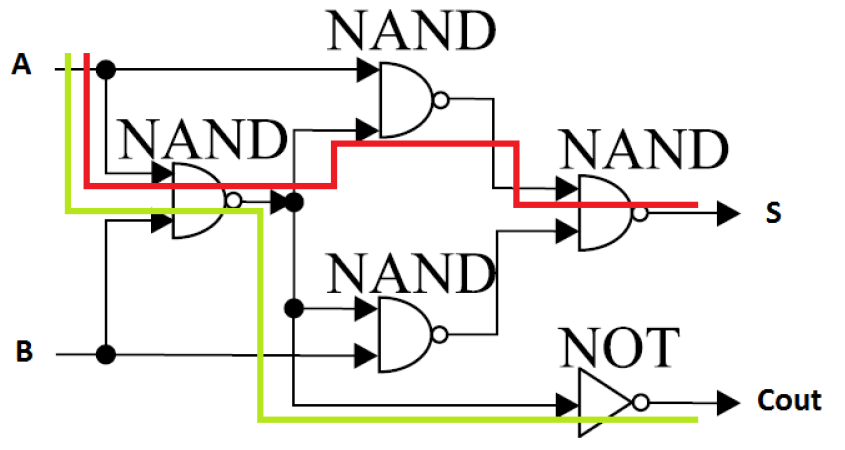
\includegraphics[scale=.36]{HA.PNG}\\
\small{Figure 1 - Half adder, NAND2 and INV gates only}\\
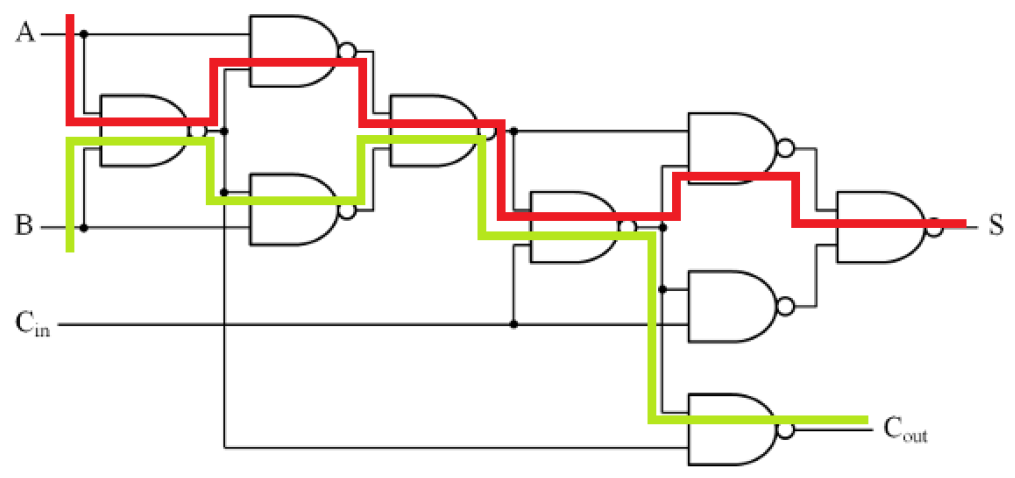
\includegraphics[scale=.34]{FA.PNG}\\
\small{Figure 2 - Full adder, NAND2 gates only}\\
\end{center}
\vspace{1em}
The green and the red lines in figures 1,2 represent the critical paths from the input to, respectively, the carry and the sum outputs. By doing these assumption on HA and FA structures, the delay and area of both blocks can be determined as shown in table 6.
\begin{center}
\begin{tabular}{|c|c|c|c|}
	\hline 
            Gate & Area & Delay IN to S & Delay IN to $C_{out}$ \\
	\hline          
	HA & $Area_{INV} + 4Area_{NAND2}$ & $3 \tau_{NAND2}$ & $\tau_{INV} + \tau_{NAND2}         $\\
	\hline 
	FA & $9Area_{NAND2}$ & $6 \tau_{NAND2}$  & $5 \tau_{NAND2}$  \\ 
	\hline 
\end{tabular} \\
\small{Table 6}
\end{center}
\newpage
\subsection{Baugh-Wooley multiplier}
The simplest way to implement a signed-inputs (2's complement number representation) array multiplier is to use the Baugh-Wooley algorithm. Starting from the operands A,B shown in the following 
\begin{center}
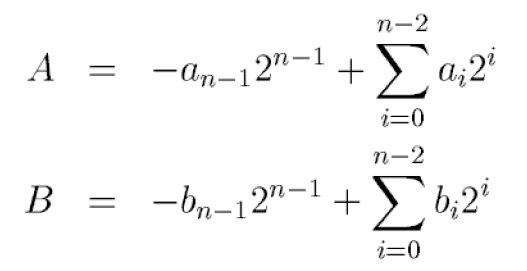
\includegraphics[scale=.34]{ab.PNG}\\
\end{center}
One can write their product as
\begin{center}
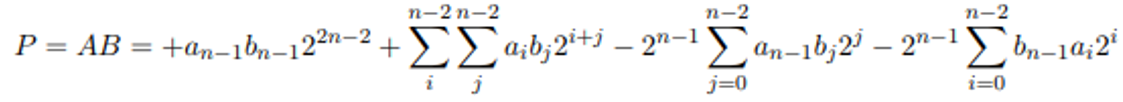
\includegraphics[scale=.42]{p.PNG}\\
\end{center}
By calling
\begin{center}
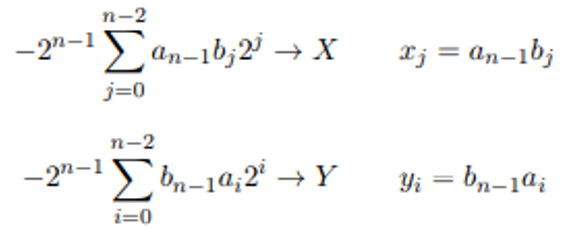
\includegraphics[scale=.34]{calling.PNG}\\
\end{center}
It is possible to see that the unrolled envelope for each power of two is as shown in figure 3.
\begin{center}
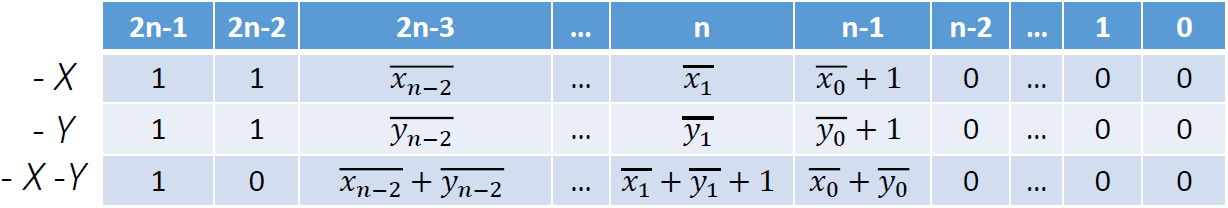
\includegraphics[scale=.38]{bw.PNG}\\
\small{Figure 3 - Baugh-Wooley algorithm}\\
\end{center}
\vspace{1em}
The final architecture for a 4x4 Baugh-Wooley multiplier is shown in figure 4.
\vspace{1em}
\begin{center}
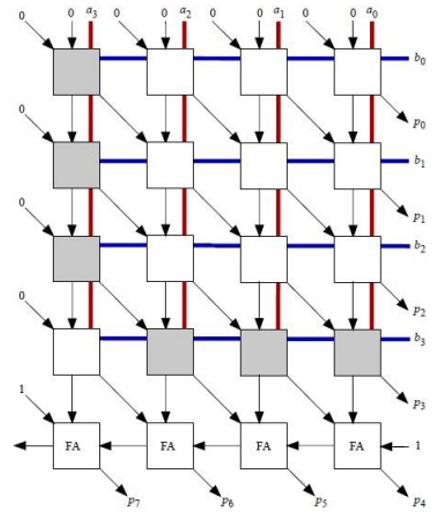
\includegraphics[scale=.54]{bwm.PNG}\\
\small{Figure 4 - 4x4 Baugh-Wooley multiplier}\\
\end{center}
\vspace{1em}
The white and grey blocks (considering also the FAs in the RCA’s chain) shown in figure 4, that compose this architecture are shown in greater detail in figure 5.
\begin{center}
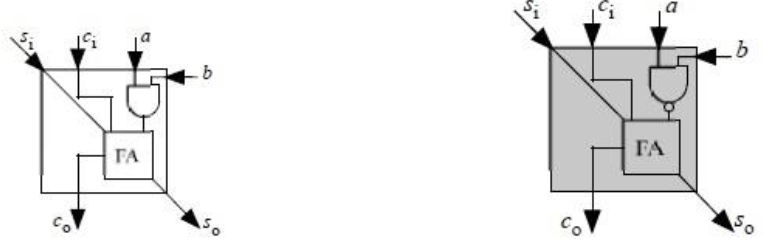
\includegraphics[scale=.48]{wgblocks.PNG}\\
\small{Figure 5 - Detail of white and grey blocks}\\
\end{center}
\vspace{1em}
It is possible to predict (table 7) how many blocks can be allocated depending on the number of bits N of the two inputs, inputs with the same width are assumed.
\begin{center}
\begin{tabular}{|c|c|}
	\hline 
            Block  & Value \\
	\hline          
	 \#Grey Blocks ($n_{GB}$) & $2 (N-1)$  \\
	\hline 
	\#White Blocks ($n_{WB}$)  &  $N^{2} - n_{GB}$ \\
	\hline 
	\#FA_{RCA} ($n_{FA}$)   & N \\
	\hline 
\end{tabular} \\
\small{Table 7}
\end{center}
The area occupied by these blocks is computed by considering a FA and a AND2 gate (obtained by the sum of the areas of a NAND2 with a INV in cascade) for the white block, and FA with a NAND2 gate for the grey one (table 8).
\begin{center}
\begin{tabular}{|c|c|}
	\hline 
            Block  & Value  \\
	\hline          
	 $area_{GB}$ & $Area_{NAND2} + Area_{FA} $ \\
	\hline 
	$area_{WB}$ & $Area_{AND2} + Area_{FA} $  \\
	\hline 
\end{tabular} \\
\small{Table 8}
\end{center}
The total area of the Baugh-Wooley is computed by summing the number of white blocks, of grey blocks and full adders, each of them multiplied by its respective area. The same considerations have been done to compute the static and the dynamic power of the structure.\\
By looking at the delay, the law that identifies the critical path, and relates it to the number of elements in the arithmetic device, can be expressed as follows:
$$ T_{CP} = \tau_{INV} + \tau_{AND2} + N \tau_{FA,s} + N \tau_{FA,c} $$
In this way, the longest path inside this structure takes into account the delay necessary to cross just one inverter, one AND2 gate and all the FAs belonging to the white and grey blocks along the vertical direction (it is possible to identify N contributions of the IN to S path of each FA). The last term in the equation is related to the needed time to cross the final RCA.
\vspace{2em}
\subsection{Even-Odd multiplier}
The Even-Odd multiplier belongs to the so called “tree multipliers”: the key idea is to use the CSA so that, starting from the partial product multiplication, a tree of reduction is created, in order to compress the information and providing two outputs. By replicating this structure until it is no more possible to obtain other partial products, a final adder can be employed to compute the product.\\
In general the components are: 
\begin{itemize}
\item Tree: made up of CSA;
\item Final 2-input adder.
\end{itemize}
With respect to the other possible configurations, the Even-Odd multiplier presents a different structure for the partial product matrix. In this case, in fact, the even and the odd partial products are summed in parallel on two distinct branches of CSA: this allows to obtain a tree with half of the depth with respect to the other standard architectures.
\vspace{1em}
\begin{center}
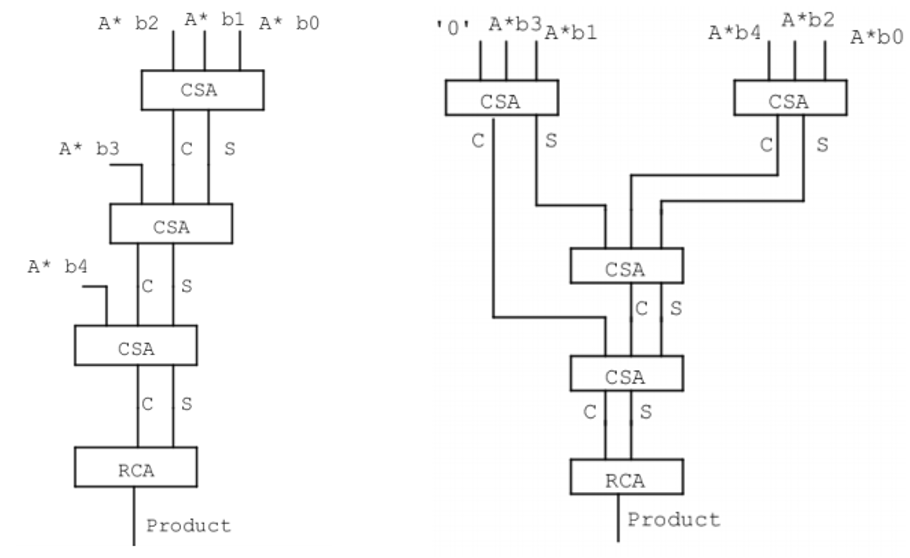
\includegraphics[scale=.40]{evenodd.PNG}\\
\small{Figure 6 - Example of even-odd multiplier}\\
\end{center}
The first part of the analysis is centered on the tree structure. The number of NAND2 gates inside a single CSA block, if N is the number of input bits of the two operands, is equal to
$$ n_{NAND2,CSA} = 9N $$
The height of the tree, instead, can be computed as
$$ h_{tree} = ceil(N) $$
In this way it is possible to calculate the number of CSA blocks:
$$ n_{CSA} = 2 h_{tree} – 2 $$
And so, starting from it, the number of NAND2 inside the tree can be computed as
$$ n_{NAND2, tree} = n_{CSA}  n_{NAND2,CSA} $$
The area related to this first part can be simply computed by multiplying the number of NAND2 gates inside the tree by the area of a single gate:
$$ area_{tree} = n_{NAND2, tree} Area_{NAND2} $$
The same consideration can be exploited to compute the contributions related to the static and dynamic power. Regarding instead the delay, the critical path can be identified in the way that connects the inputs to the output passing through the entire tree. In the example shown in figure 7 it has been assumed to have a final RCA. The critical path can be computed as
$$ \tau_{tree} = h_{tree} \tau_{FA,c} $$
\vspace{1em}
\begin{center}
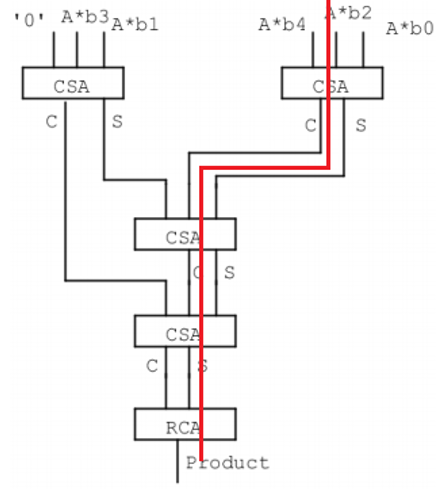
\includegraphics[scale=.42]{evenoddtcp.PNG}\\
\small{Figure 7 - Example of critical path in the even-odd multiplier}\\
\end{center}
\vspace{2em}
\subsection{Modified Booth Multiplier}
MBE is a Radix-4 approach, it halves the number of partial products with respect to the standard version of Booth Encoding, which is a Radix-2 approach. Normally it would be required to fully sign-extend the 2's complement partial product representations, but exploiting Roorda's approach it is possible to avoid such overhead, hence reducing considerably the number of compressors (full adders /half adders) in the adder plane.\\
The partial products $p_j$ are selected based on three bits of operand $b$, namely $b_{2j+1}$, $b_{2j}$ and $b_{2j-1}$. The encoding is shown in figure 8.
\vspace{1em}
\begin{center}
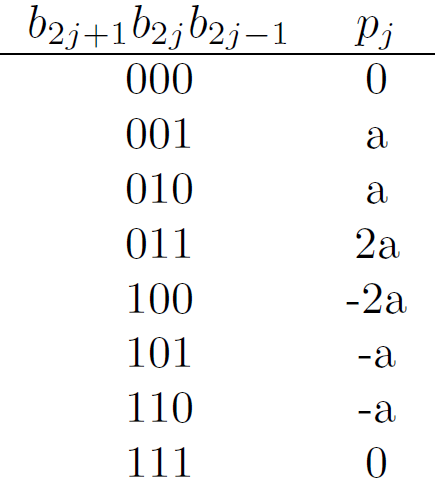
\includegraphics[scale=.30]{mbe.PNG}\\
\small{Figure 8 - Modified Booth Encoding.}
\end{center}
\vspace{1em}
Instead of directly generating all the possible partial products as 0, a, 2a, -a and -2a depending on multiplicand b triplet of bits, the expression describing partial products (which can be derived from direct inspection of figure 8) is more complex
in MBE than in Radix-2 solutions, namely
\begin{center}
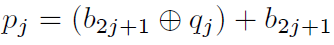
\includegraphics[scale=.42]{form1.PNG}\\
\end{center}
where
\begin{center}
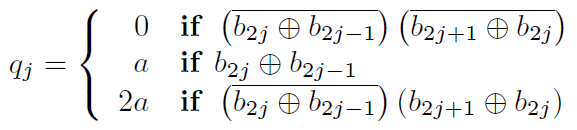
\includegraphics[scale=.42]{form2.PNG}\\
\end{center}
The model was simplified w.r.t. theory, but the error in terms of employed resources/power is negligible, at least w.r.t. the lower-level modeling where only NAND2-INV gates were considered to be the building blocks of more complex structures.




\newpage
\section{Reduction tree}
The main goal of a reduction tree is to reduce the sum of N operands to the sum of just two operands, that can be handled by a conventional (possibly fast) adder. Reduction trees are based on the carry-save approach, that is faster w.r.t. the carry-propagate approach. Blocks such as full adders and half adders are not seen anymore as basic addition blocks, but just as compressors.\\
In this work, as mentioned in section 1, it is possible to build multipliers properly choosing the partial products generation circuit, the reduction tree and the final adder. Regarding the reduction tree the user has the possibility to choose between Wallace and Dadda strategies. This choice is of course not allowed in case of special multipliers such as array multiplier (that is called "Baugh-Wooley" if signed operands are considered) or even-odd multiplier.
\vspace{2em}
\subsection{Wallace}
Wallace  reduction  tree  is  based  on  an  ASAP  philosophy. As opposed to Dadda reduction tree, the number of dots in each column is reduced at the earliest opportunity. Since the standard compressors are full adders and half adders, with a maximum compression ratio of 1.5 in the case of FAs, in each reduction step it's not possible to reduce the number of dots in each column with a factor higher than 1.5.
A consequence of the massive resource use is the reduction 
of the final (two-operand) adder width, that ideally should be a positive feature in terms of critical path, but it's actually not true: in any case Dadda reduction tree is faster.\\
\vspace{1em}
\begin{center}
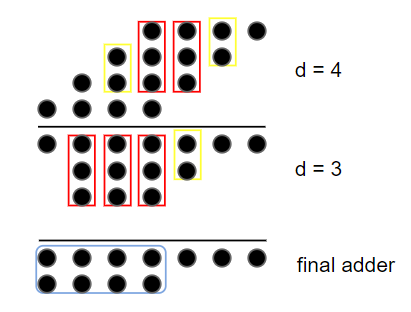
\includegraphics[scale=.46]{wallace.PNG}\\
\small{Figure 9 - 4x4 multiplication, Wallace reduction tree}
\end{center}
\vspace{1em}
In figure 9 an example of 4x4 multiplication exploiting Wallace strategy is shown. Yellow rectangles determine an HA, red rectangles determine a FA.\\
The approach used to determine the total number of compressors and the critical path of the reduction tree is similar to the one explained in section 4.2. The main difference is that instead of using the minimum amount of resources to reach a desired height in the following reduction step, now a parameter "coverable\_dots" is associated to each column, so that the proper amount of compressors is used. For instance if $coverable\_dots = 6$, if and only if the dots are actually available 2 FAs will be used. When the column weight is equal or greater than $2^{N+1}$, the number of coverable dots will be reduced by one while going from one column to the following one (least significant to most significant).
\vspace{2em}
\subsection{Dadda}
Dadda reduction tree is based on an ALAP philosophy. At each reduction stage it employs the minimum number of compressors so that the number of dots in each column would not exceed the one of the correspondent Wallace tree. Analytically, considering a target depth $d_0 = 2$ for the final adder, the respective depths at the previous reduction steps will be $$ d_{j+1}=floor(1.5d_j)$$ In this way the number of stages will be the same as in the Wallace tree, but with less resources employed. The final adder will be instead slightly wider w.r.t. Wallace strategy, but overall Dadda reduction tree is slightly faster (for all operand sizes) and requires fewer gates (for all but the smallest operand sizes). Dadda reduction tree is faster even though the final CPA width is larger w.r.t. Wallace reduction tree CPA, in which S bits of the final sum (S is the number of reduction stages) was already computed inside the tree. An example of a 4x4 multiplication, represented in dot notation, is shown in figure 10. Yellow rectangles represent the use of HAs, while the red ones represent the use of FAs.
\vspace{1em}
\begin{center}
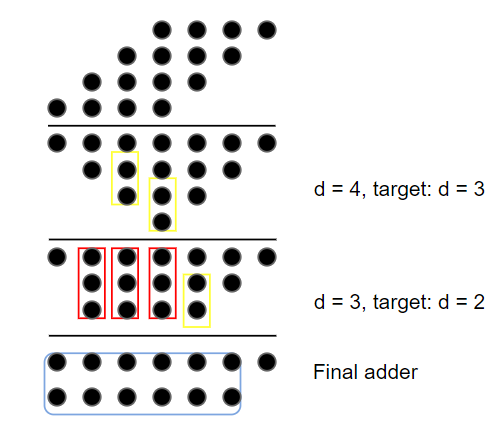
\includegraphics[scale=.48]{dadda4x4.PNG}\\
\small{Figure 10 - 4x4 multiplication, Dadda reduction tree}
\end{center}
\vspace{1em}
In order to find the Dadda reduction tree critical path the methodology described in [4] is used. Each dot of the typical dot notation is replaced, inside a matrix, with a number that represents the delay of the bit in that particular position.
An iterative algorithm reduces column by column the tree, stage after stage, where in each stage a desired height is specified into a pre-computed vector. Each column is analyzed sequentially,
starting from the least significant and moving to the most significant one. The cycle (analysis of each column, in each reduction stage) is carried out
until the matrix is reduced to just two rows.
When a column must be reduced, a FA is used only if that specific column must compress more than one bit. Both the sum and the carry delays are propagated vertically, to the next stage: the sum
in the same column, while the carry in the next (higher weight) column.
\newpage
\section{Final two-operand adder}
In this section the possible user selectable two-operand adders are described. It is possible to choose a slow final adder such as the standard RCA (Ripple-Carry Adder), or a faster solution such as the CLA (Carry-Lookahead Adder) or a parallel-prefix approach adder (Ladner-Fischer, Brent-Kung, Kogge-Stone).
\vspace{1em}
\subsection{RCA}
It is the simplest solution to add two N-bit numbers, since it is just a cascade of full adders. Its name derives from the fact that each carry bit "ripples" to the next full adder, hence it is a quite simple but slow solution. Note that the first (and only the first) full adder may be replaced by a half adder (under the assumption that $C_{in} = 0$).\\
The model of such an adder is quite simple, the only consideration that has been done is related to its width: in case of Wallace reduction tree the RCA will be characterized by a width reduced by the value S (number of reduction stages) w.r.t. Dadda reduction tree, since those bits are already computed inside the reduction tree.\\
The model is summarized in table 9, note that N changes whether in the previous step there was a Wallace or Dadda reduction tree.
\begin{center}
\begin{tabular}{|c|c|}
	\hline 
            Parameter  & Value \\
	\hline          
	 $area_{RCA}$ & $n_{NAND2, RCA} area_{NAND2} $ \\
	\hline 
	$\tau_{RCA}$ & $N \tau_{FA,c}$ \\
	\hline 
	$Ps_{RCA}$ & $n_{NAND2, RCA} Ps_{NAND2} $  \\
	\hline 
	$Pdyn_{RCA}$ & $n_{NAND2, RCA} Pdyn_{NAND2} $    \\
	\hline 
\end{tabular} \\
\small{Table 9}
\end{center}
\vspace{1em}
\subsection{CLA}
The CLA tree structure (figure 11) is made of "A" blocks and "B" blocks, whose operations are specified in the same figure.
\vspace{1em}
\begin{center}
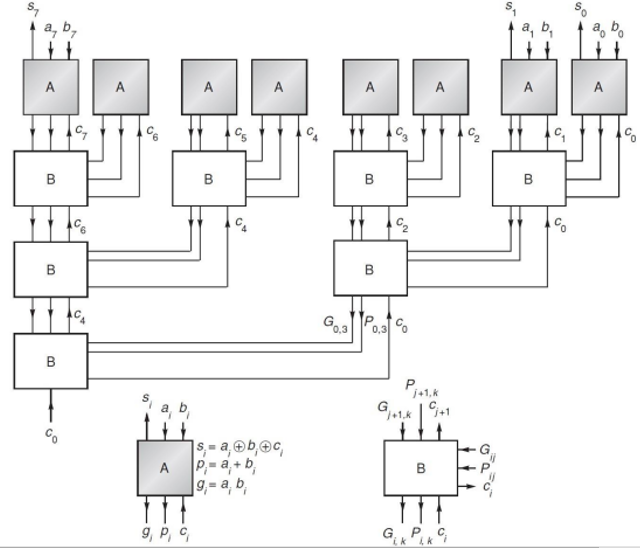
\includegraphics[scale=.50]{clatree.PNG}\\
\small{Figure 11 - CLA tree example with details on "A","B" blocks}
\end{center}
\vspace{1em}
It’s possible to determine all the parameters by firstly considering the number of A blocks ($N_{A}$) equal to N, and of B blocks ($N_{B}$) equal to N-1. The parameters are summarized in table 10.
\begin{center}
\begin{tabular}{|c|c|}
	\hline 
            Parameter  & Value  \\
	\hline
            $n_{NAND2, A}$ & $ n_{NAND2,GEN_A} + n_{NAND2,PROP_A} + n_{NAND2,S_A} $ \\
            \hline  
            $n_{INV, A}$ & $ n_{INV,GEN_A} + n_{INV,PROP_A} $ \\
            \hline     
            $n_{NAND2, B}$ & $ n_{NAND2,GEN_B} + n_{NAND2,PROP_B} + n_{NAND2,C_B} $ \\
            \hline  
            $n_{INV, B}$ & $ n_{INV,GEN_B} + n_{INV,PROP_B} + n_{INV,C_A} $  \\
            \hline     
	 $area_{CLA}$ & $(n_{NAND2, A}+ n_{NAND2, B}) area_{NAND2} + (n_{INV, A}+ n_{INV,    B}) area_{INV}  $ \\
	\hline 
	$Ps_{CLA}$ & $(n_{NAND2, A}+ n_{NAND2, B}) Ps_{NAND2} + (n_{INV, A}+ n_{INV,    B}) Ps_{INV}  $\\
	\hline 
	$Pdyn_{CLA}$ & $(n_{NAND2, A}+ n_{NAND2, B}) Pdyn_{NAND2} + (n_{INV, A}+ n_{INV,    B}) Pdyn_{INV}  $\\
	\hline 
\end{tabular} \\
\small{Table 10}
\end{center}
Regarding the delay parameters, the discussion is slightly more complex. For that reason it’s necessary to analyze the paths associated to the A and B blocks. In fact each block is composed by different gates that have to be crossed. So there are various delays related to:
\begin{itemize}
\item Generate the result in the A block: $\tau_{generate,A}$, it is equal to the time needed to cross the A block from top to bottom ($\tau_{A,down}$);
\item Propagate the result in the A block: $\tau_{propagate,A}$;
\item Sum computation in A block: $\tau_{sum,A}$, it is equal to the time needed to cross the A block in the up direction ($\tau_{A,up}$);
\item Generate the result in B block: $\tau_{generate,A}$, it is equal to the time needed to cross the B block from top to bottom direction ($\tau_{B,down}$);
\item Propagate the result in B block: $\tau_{propagate,B}$;
\item Carry computation: $\tau_{carry,B}$, it is equal to the time needed to cross the B block in the up direction ($\tau_{B,up}$);
\end{itemize}
By knowing these contributions it is possible to obtain the total amount of the delay necessary to cross the critical path as
$$ \tau_{CLA} = \tau_{A,down} + (log2(2*N-2) - 1) \tau_{B,down} + (log2(2*N-2)) \tau_{B,up} +\tau_{A,up}$$
\vspace{2em}
\subsection{Parallel-Prefix approach}
Three types of parallel-prefix approach adders have been implemented: Ladner-Fischer, Brent-Kung and Kogge-Stone. The following considerations are valid for all the three adders, in particular:
\begin{itemize}
    \item Generate/propagate signal computation blocks are composed by 2 AND2 and 1 OR2 gates, that correspond to 7 NAND2 gates. For simplicity these blocks will be called "black" blocks;
    \item Sum computation blocks are composed by 1 AND2 and 1 OR2 gates, that correspond to 5 NAND2 gates. The number of these blocks is $2 N -2$ (actually $2N-i$ in case of Wallace reduction tree). For simplicity these blacks will be called "grey" blocks;
    \item The critical path along the latter two blocks is equal to $ 4 \tau_{NAND2}$;
    \item The number of NAND2 gates in the prefix (generate/propagate signals computation) stage is $num_{precomputation} = (2N-2)(6)$ , while the number of NAND2 gates in the sum/carry-out computation network will be equal to $num_{result}= (2N-2)4 + 5$
\end{itemize}
What's in the middle of the parallel prefix graph of course depends on the specific implementation.
\vspace{2em}
\subsubsection{Ladner-Fischer adder}
The number of NAND2 gates of the Ladner-Fischer network can be computed by multiplying by 7 (2 AND2 and 1 OR2 gates correspond to 7 NAND2 gates) the total number of group generate/group propagate signal computation blocks ("black" blocks) , and by 5 the number of "grey" blocks as follows
$$ N_{NAND2,LF} = 7 (\frac{2N-2}{2} log_2 (2N -2)) + 5 (2N-2)$$
The total number of NAND2 gates used for the final two-operand adder will include this quantity and the two contributions that are true for whatever parallel-prefix network:
$$ N_{NAND2,total} = num_{precomputation} + N_{NAND2,LF} + num_{result} $$
With this value it's possible to trivially compute the area, static and dynamic power of the Ladner-Fischer adder.\\
Considering instead the critical path, it is possible to compute it simply by applying the following equation:
$$T_{cp} = log_2(2N-2) \tau_{"black"block} + \tau_{"grey"block} + 2 \tau_{XOR2}$$
\vspace{1em}
\begin{center}
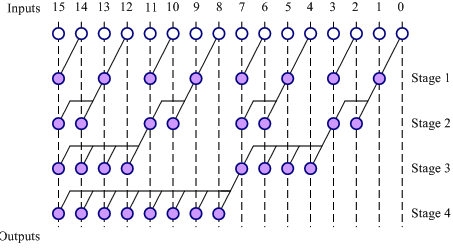
\includegraphics[scale=.80]{ladner.PNG}\\
\small{Figure 12 - 16-bit Ladner-Fischer adder}
\end{center}
\vspace{1em}
The Ladner-Fischer adder, shown in figure 12, is characterized by a very low depth (ideally fast), but also by high-fanout nodes that will translate to slower speed, especially for large width additions. The high-fanout problem is not visible in the results since it was not included into the simplified model.
\newpage
\subsubsection{Brent-Kung adder}
The only difference w.r.t. Ladner-Fischer adder, or other adders based on the parallel-prefix approach, is related to the number of "black" blocks and of course on the height of the adder. The number of "black" blocks $ num_{"black"blocks,BK} $ can be computed as follows
$$ num_{"black"blocks,BK} = 2(2N-2)-2-log_2 (2N-2)$$
hence one can compute the number of NAND2 gates into the Brent-Kung-specific portion of the adder as
$$ N_{NAND2,BK} = 7 num_{"black"blocks,BK}  + 5 (2N-2)$$
and finally the total number of NAND2 gates into the Brent-Kung adder will be 
$$ N_{NAND2,total} = num_{precomputation} + N_{NAND2,BK} + num_{result} $$
As in section 4.3.1 one can easily compute the area, static and dynamic power of the adder starting from the $ N_{NAND2,total}$ quantity.
The critical path can be computed as follows
$$ T_{cp} = (2log_2(2N-2)-2) \tau_{"black"block} + \tau_{"grey"block} + 2 \tau_{XOR2}$$
\vspace{1em}
\begin{center}
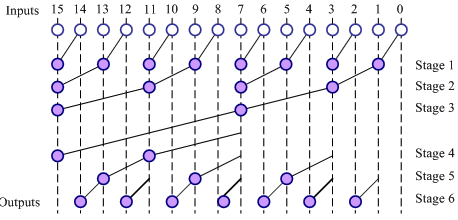
\includegraphics[scale=.80]{brent.PNG}\\
\small{Figure 13 - 16-bit Brent-Kung adder}
\end{center}
\vspace{1em}
The Brent-Kung adder, shown in figure 13, solves the problem of high-fanout seen in the Ladner-Fischer adder, at the expense of a larger depth, hence it is (ideally) slower. It is also characterized by a lower complexity.
\vspace{2em}
\subsubsection{Kogge-Stone adder}
One can repeat the same steps as in sections 4.3.1  and 4.3.2, the only parameters that change are the following:
$$ num_{"black"blocks,KS} = (2N-2)log_2 (2N-2) - (2N-2) +1$$
$$ T_{cp} = log_2(2N-2) \tau_{"black"block} + \tau_{"grey"block} + 2 \tau_{XOR2}$$
With the first formula one can easily derive the total number of NAND2 gates of the Kogge-Stone adder, to then be able to compute the area, static and dynamic power. The second formula can be directly employed to compute the critical path and of course the maximum operating frequency (referring just to the adder).\\
\vspace{1em}
\begin{center}
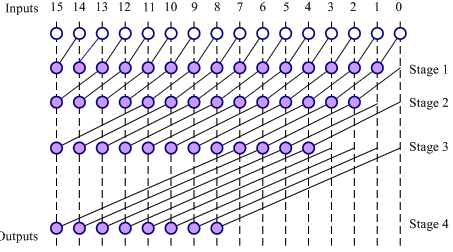
\includegraphics[scale=.80]{kogge.PNG}\\
\small{Figure 14 - 16-bit Kogge-Stone adder}
\end{center}
\vspace{1em}
The Kogge-Stone adder, shown in figure 14, solves the problem of high-fanout seen in the Ladner-Fischer adder and also guarantees the same height, hence ideally this architecture is the fastest, but also the most expensive in terms of area.
\newpage
\section{Results and possible improvements}
In this section several use cases (possible user-defined heterogeneous multipliers) are investigated and compared. Finally, some possible improvements are discussed.
\vspace{2em}
\subsection{Example A: Baugh-Wooley multiplier}
As an example a width of $N = 155$ was chosen, then Baugh-Wooley multiplier was selected by imposing $a=1$. This multiplier is simply an array multiplier with the capability of working with signed 2's complement numbers. It is characterized by a special architecture, hence the user is not asked to specify the reduction tree and final two-operand adder types. The results are shown in figure xxxx.
\vspace{1em}
\begin{center}
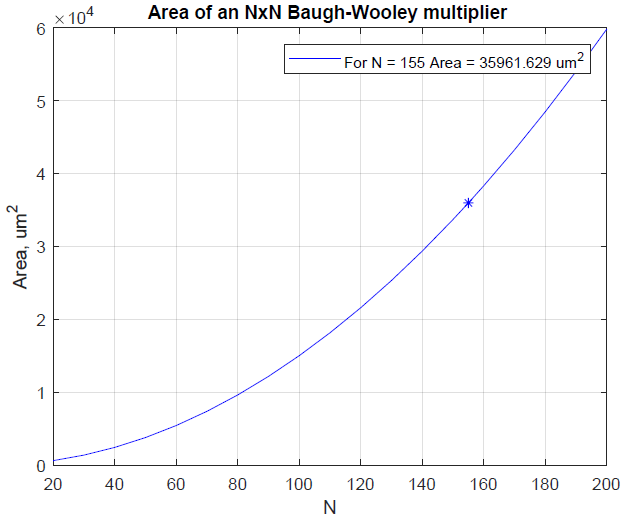
\includegraphics[scale=.48]{area_bw.PNG}
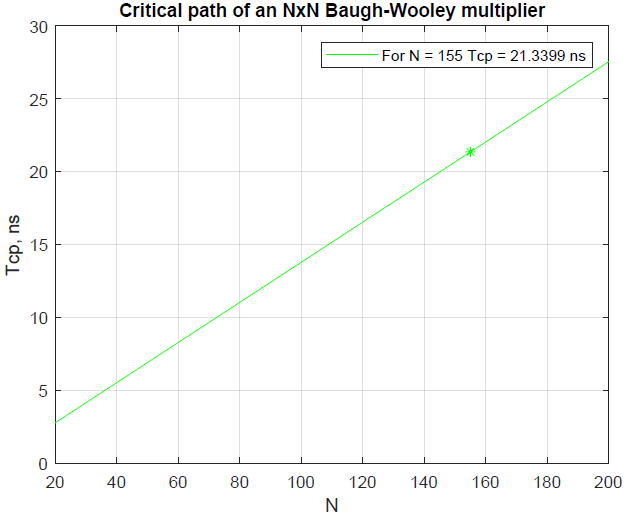
\includegraphics[scale=.48]{tcp_bw.PNG}\\
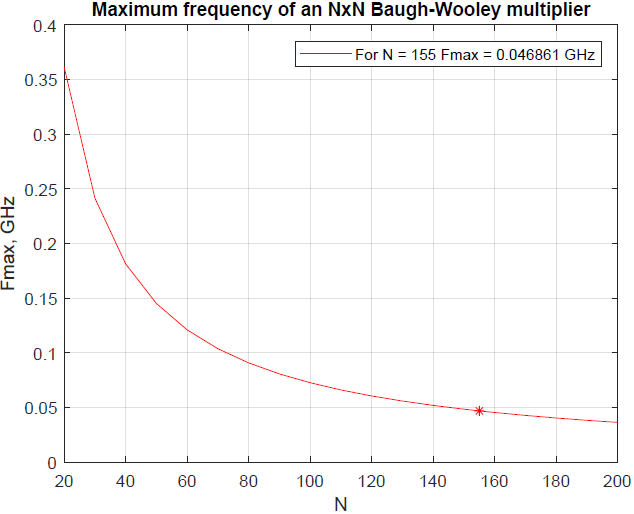
\includegraphics[scale=.48]{fmax_bw.PNG}
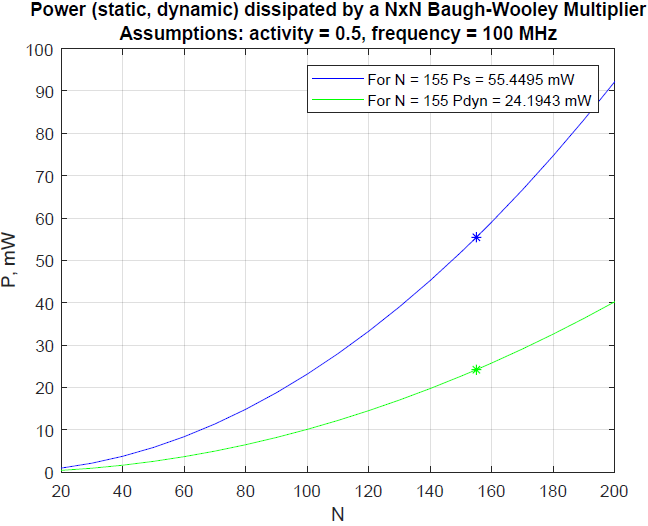
\includegraphics[scale=.48]{power_bw.PNG}
\small{Figure xxxx - Baugh-Wooley multiplier. Values for multiplier width $N=155$ are explicitly shown}
\end{center}
\vspace{1em}
The Baugh-Wooley multiplier is characterized, as expected, by a quite long critical path due to the carry-propagate philisophy. For a multiplier width of $N = 155$ the maximum operating frequency is lower than 47 MHz.\\
The dynamic power was estimated considering an activity of 0.5 and a reference operating frequency of 100 MHz, that is actually higher w.r.t. what the multiplier can actually achieve. A possible improvement to avoid this looseness is briefly discussed in section 6.5.
\vspace{3em}
\subsection{Example B: Dadda multiplier with RCA}
Again $N = 155$ was chosen. The Dadda multiplier was selected by imposing the $a$ parameter equal to 2, then the Ripple-Carry adder was selected by imposing the $c$ parameter equal to 1. Of course in this case the user is not asked to insert the $b$ parameter, since it is related to the reduction tree typology that is already implied by the $a$ parameter. The results are shown in figure xxxx.
\vspace{1em}
\begin{center}
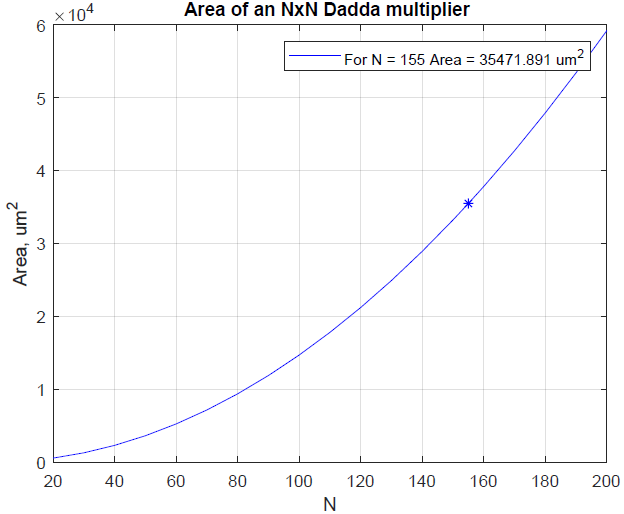
\includegraphics[scale=.48]{area_dadda_rca.PNG}
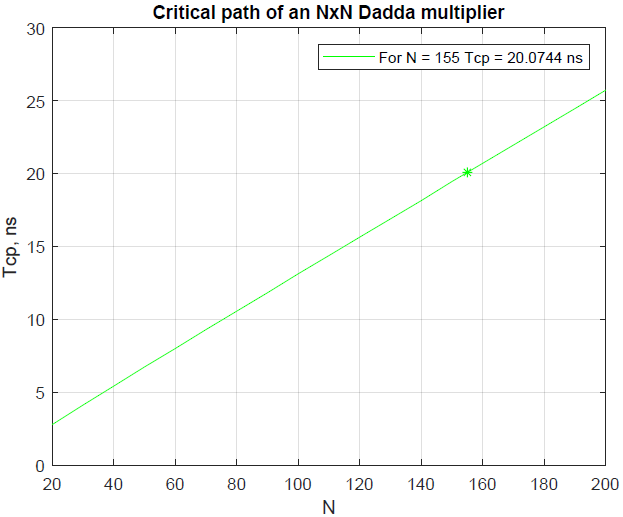
\includegraphics[scale=.48]{tcp_dadda_rca.PNG}\\
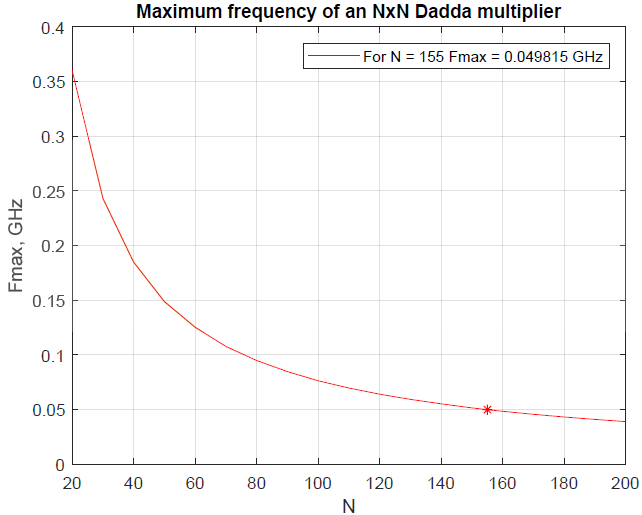
\includegraphics[scale=.48]{fmax_dadda_rca.PNG}
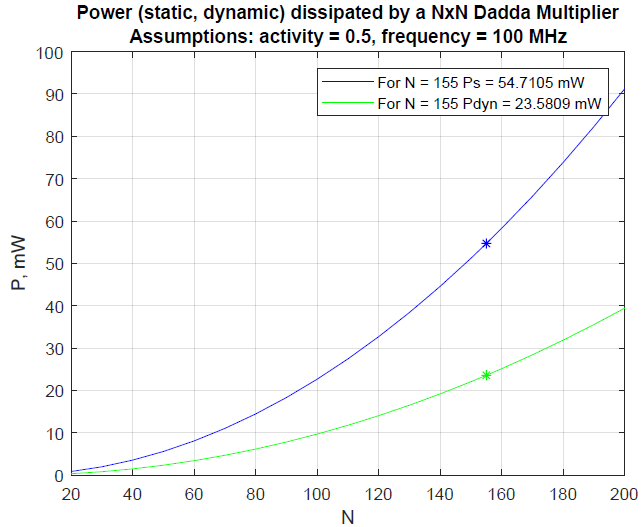
\includegraphics[scale=.48]{power_dadda_rca.PNG}
\small{Figure xxxx - Dadda multiplier, RCA as final adder. Values for multiplier width $N=155$ are explicitly shown}
\end{center}
\vspace{1em}
W.r.t. Baugh-Wooley multiplier (section 6.1) the Dadda multiplier with a Ripple-Carry adder as final two-operands adder shows very similar performance. The improvement in terms of area and static power is around 1.3\%, maximum frequency improved of about 6.3\%.
The critical path still increases linearly with multiplier width N.
\newpage
\subsection{Example C: Dadda multiplier with Ladner-Fischer (parallel prefix) adder}
Again $N = 155$ was chosen. Again the Dadda multiplier was selected by imposing the $a$ parameter equal to 2, then the Ladner-Fischer adder (parallel prefix approach) was selected by imposing the $c$ parameter equal to 2. The results are shown in figure xxxx.
\vspace{1em}
\begin{center}
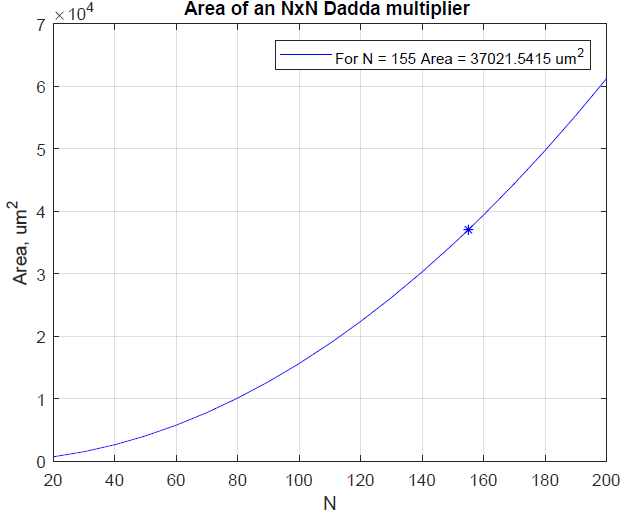
\includegraphics[scale=.48]{area_dadda_pp_lf.PNG}
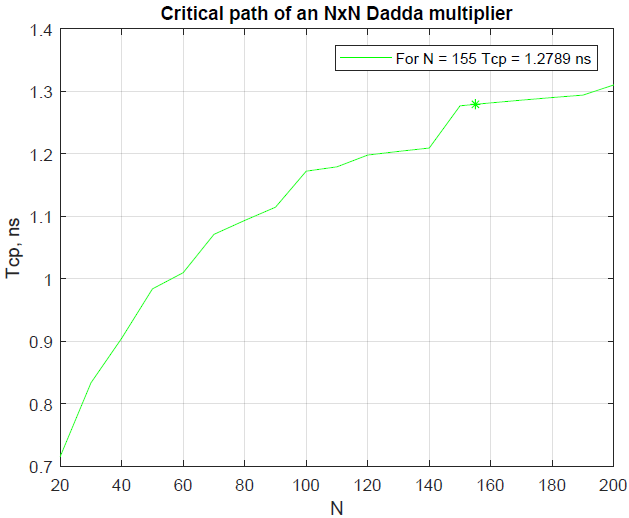
\includegraphics[scale=.48]{tcp_dadda_pp_lf.PNG}\\
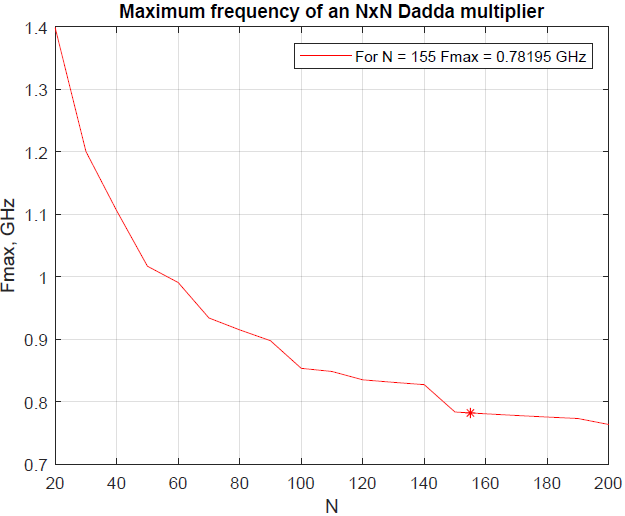
\includegraphics[scale=.48]{fmax_dadda_pp_lf.PNG}
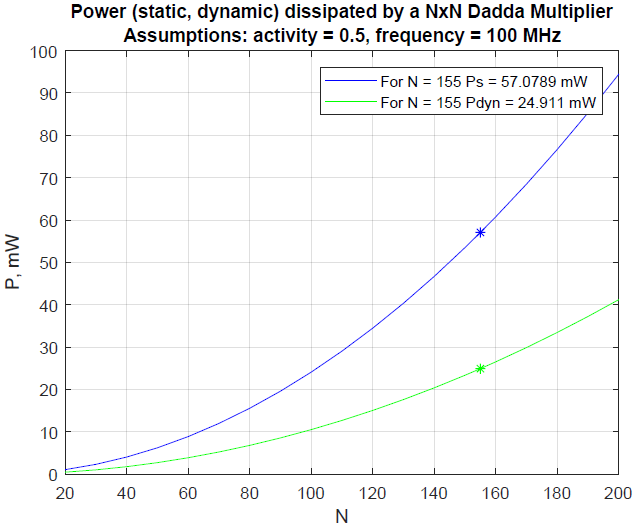
\includegraphics[scale=.48]{power_dadda_pp_lf.PNG}
\small{Figure xxxx - Dadda multiplier, Ladner-Fischer as final adder. Values for multiplier width $N=155$ are explicitly shown}
\end{center}
\vspace{1em}
With a fast adder, in this case Ladner-Fischer network, since it is characterized by a logarithmic critical path dependency on multiplier width N, the performance improves dramatically w.r.t. example B (section 6.2), especially for high values of N.\\
W.r.t. the RCA case the maximum frequency improves massively, at the cost of a slightly higher complexity and of course higher static power. It is possible to increase the operating frequency ( by default set to 100 MHz), hence the dynamic power would also increase dramatically.
\newpage
\subsection{Example D: MBE multiplier with Dadda reduction tree and CLA final adder}
The last example better shows the potential of the script: it is possible to estimate the performance of unusual multipliers, such as MBE ( Modified Booth Encoding) multiplier, with Dadda reduction tree and CLA (Carry Look-Ahead) final adder. Again, for the sake of comparison, $N = 155$ was chosen as multiplier parallelism. Then the specified parameters to "build" such a multiplier were $a=4$, $b=1$, $c=5$. The results are shown in figure xxxx.
\vspace{1em}
\begin{center}
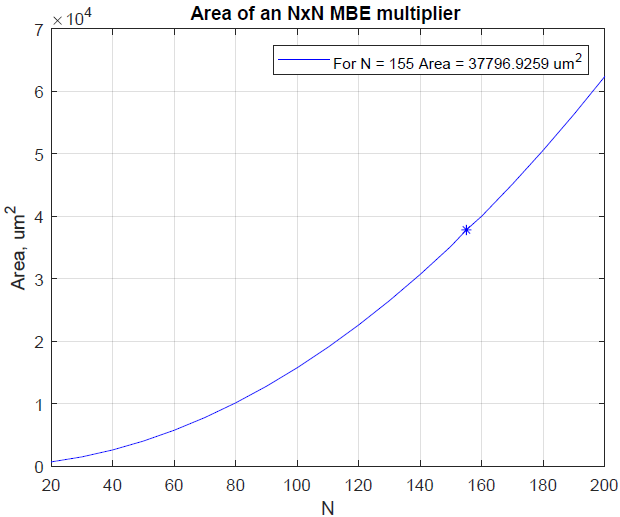
\includegraphics[scale=.48]{area_mbe.PNG}
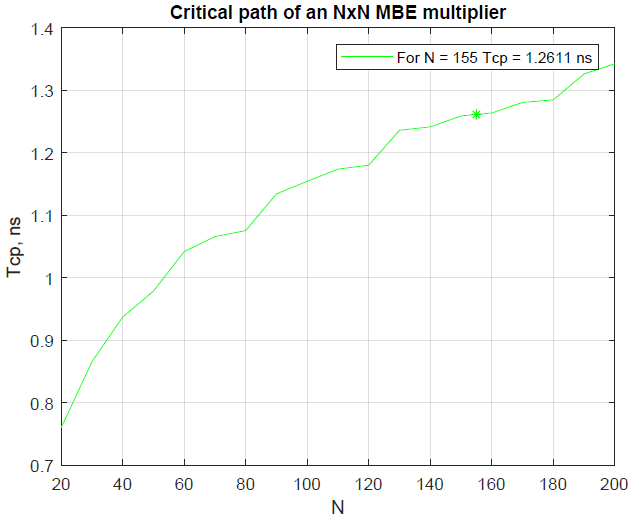
\includegraphics[scale=.48]{tcp_mbe.PNG}\\
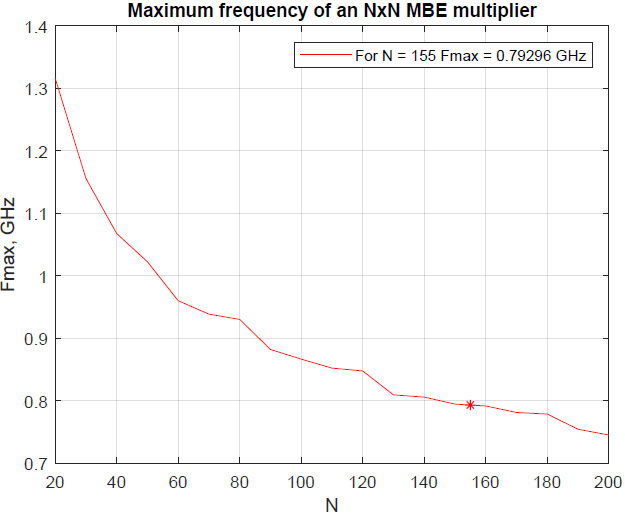
\includegraphics[scale=.48]{fmax_mbe.PNG}
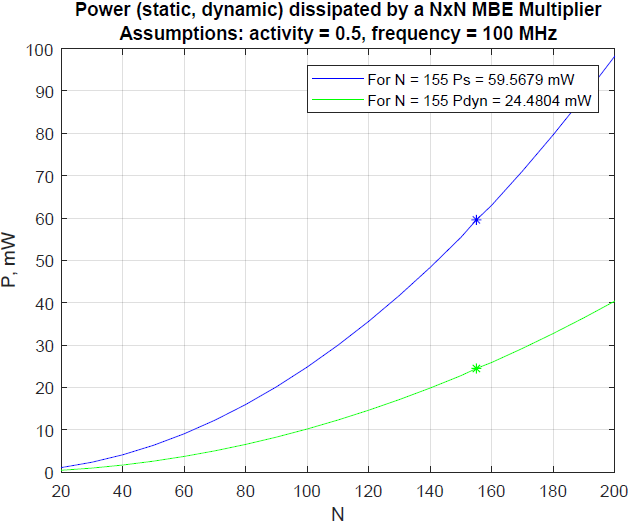
\includegraphics[scale=.48]{power_mbe.PNG}
\small{Figure xxxx - MBE multiplier, Dadda reduction tree and CLA as final adder. Values for multiplier width $N=155$ are explicitly shown}
\end{center}
\vspace{1em}
With this multiplier one can see how it is possible to stretch even more the maximum frequency at the cost of a slightly higher complexity. With a Ladner-Fischer final adder it would be possible to improve even further the maximum frequency, of course paying in terms of area.
\vspace{2em}
\newpage
\subsection{Possible improvements}
One can possibly improve the script by refining the employed models, especially the Wallace one, or by adding new models to further enhance flexibility.\\
Another improvement would be choosing as operating frequency the maximum frequency instead of the reference one (100 MHz) for a better dynamic power estimation. This would be a bit tricky since the dynamic power is computed (like the other output parameters) three times, once for each module (partial product generation network, reduction tree and final adder), and of course each module has a different maximum operating frequency.
\newpage
\appendix
\section{Appendix}
\footnotesize
\lstinputlisting{mpy.m}
\end{document}